\documentclass{article}
\usepackage{graphicx} % Required for inserting images

\title{Group 5 Project Report}
\author{Ashley Björs,Elliot Bodin,Daniel Rytenberg,Jonas Gerne}
\date{Febuary 2024}

\begin{document}
\maketitle




\clearpage
\section{Waveforms}

\begin{figure}[h]
    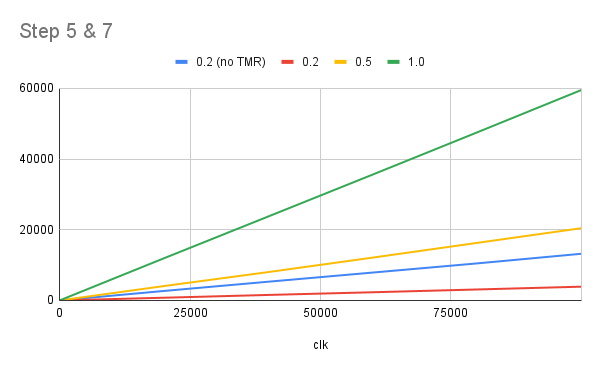
\includegraphics[width=5cm]{{images/Step 5 & 7.png}}
    \centering
    \caption{This is the LUT list of step 1}
\end{figure}
\begin{figure}[h]
    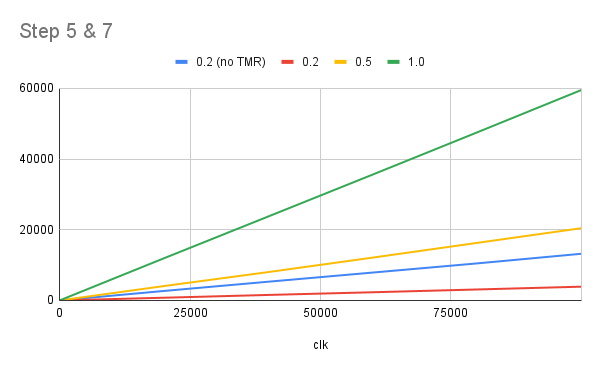
\includegraphics[width=5cm]{{images/Step 5 & 7.png}}
    \centering
    \caption{This is the LUT list of step 1}
\end{figure}
\begin{figure}[h]
    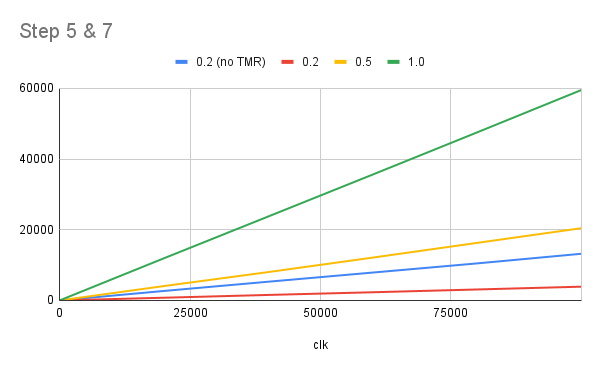
\includegraphics[width=5cm]{{images/Step 5 & 7.png}}
    \centering
    \caption{This is the LUT list of step 1}
\end{figure}
\begin{figure}[h]
    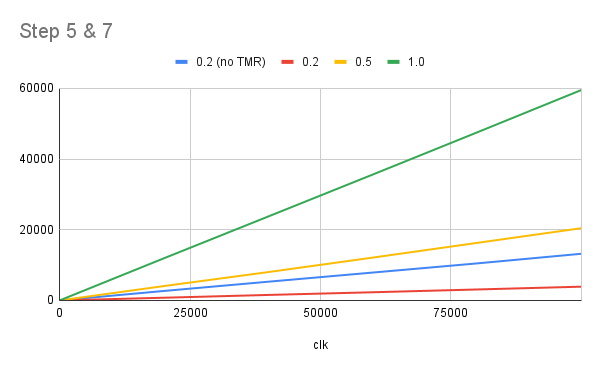
\includegraphics[width=5cm]{{images/Step 5 & 7.png}}
    \centering
    \caption{This is the LUT list of step 1}
\end{figure}
\begin{figure}[h]
    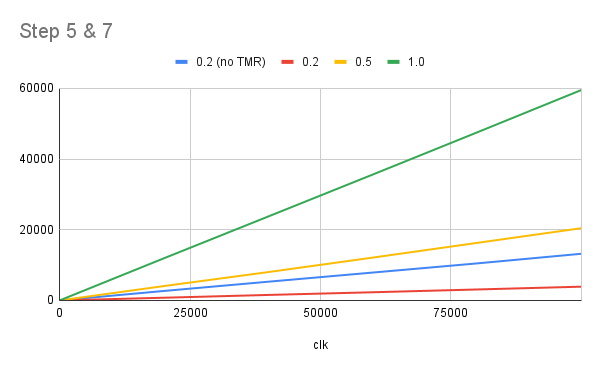
\includegraphics[width=5cm]{{images/Step 5 & 7.png}}
    \centering
    \caption{This is the LUT list of step 1}
\end{figure}
\begin{figure}[h]
    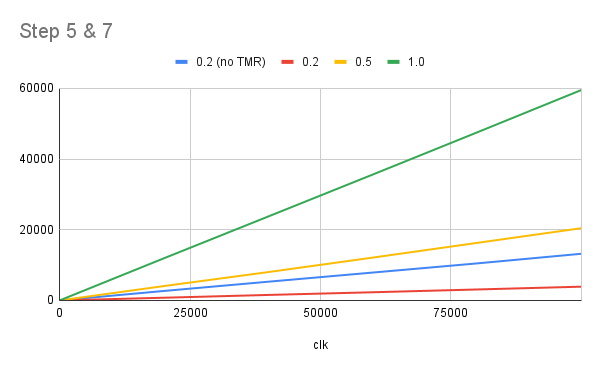
\includegraphics[width=5cm]{{images/Step 5 & 7.png}}
    \centering
    \caption{This is the LUT list of step 1}
\end{figure}
\begin{figure}[h]
    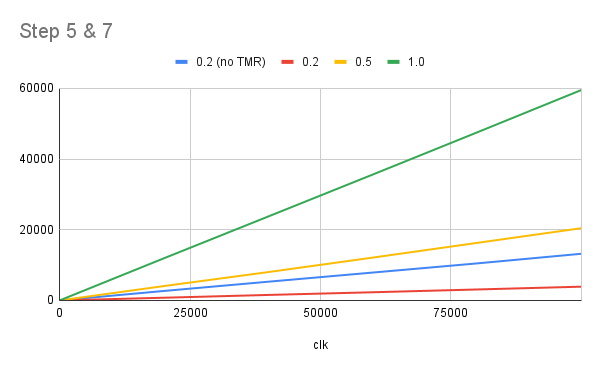
\includegraphics[width=5cm]{{images/Step 5 & 7.png}}
    \centering
    \caption{This is the LUT list of step 1}
\end{figure}

\clearpage
\section{Graph}


\begin{figure}[h]
    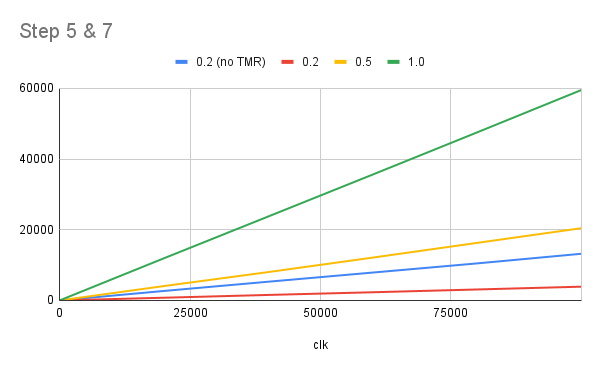
\includegraphics[width=\linewidth]{{images/Step 5 & 7.png}}
    \centering
    \caption{The Y-axis being the number of errors. The X-Axis being the nr of clock cycles}
\end{figure}

\end{document}
